\documentclass[11pt]{article}
\usepackage[utf8]{inputenc}
\usepackage[italian]{babel}
\usepackage{amssymb}
\usepackage{verbatim}
\usepackage{amsfonts}
\usepackage{amsmath}
\usepackage{amsthm}
\usepackage{float}
\usepackage{xcolor}
\usepackage{graphicx}
\graphicspath{ {./images/} }

\title{Titolo}
\author{Daniele De Micheli}
\date{2019}

\renewcommand*\contentsname{\textit{Indice}}

%presettaggio per teoremi e assiomi/definizioni%

\newtheorem*{nome}{teorema}

%fine%

\begin{document}

\maketitle
\tableofcontents

\part{Prima parte}

\section{Processi}
\subsection{Concetto di processo}
I processi rappresenta la prima e più importante astrazione a livello software per un sistema operativo. Un SO esegue infatti un certo numero di programmi contemporaneamente; ogni programma rappresenta un \textbf{processo}, e questi processi vengono eseguiti in maniera sequenziale.
Un processo è composto da diverse parti:
\begin{itemize}
	\item Lo stato dei registri del processore, incluso il program counter.
	\item Il codice del programma (\textit{text section}) - PID -.
	\item Lo \textbf{stack} delle chiamate, contenente parametri, variabili locali e indirizzo di ritorno (compreso lo \textit{stack pointer}).
	\item La \textbf{data section}, contenente le variabili globali.
	\item Lo \textbf{heap}, contenente la memoria allocata dinamicamente durante l'esecuzione. Per esempio, in Java viene indicata con \emph{New}, in C con \emph{malloc}.
	\item Altre risorse acquisite (es. file aperti).
\end{itemize}
Un porgramma è un'entità passiva (file eseguibile su disco), un processo è un'entità attiva(è un programma in esecuzione). Un progrmma "diventa" un processo quando viene caricato nella memoria centrale. Esso può generare diversi processi:
\begin{enumerate}
	\item Molti utenti eseguono lo stesso programma
	\item Uno stesso programma ...
\end{enumerate}

La memoria di un processo è divisa tra stack e heap. Dopo lo heap c'è la sezione \textbf{data} (e in linux anche la sezione \textbf{bss}) e successivamente la sezione \textbf{text}.

\begin{figure}[ht]
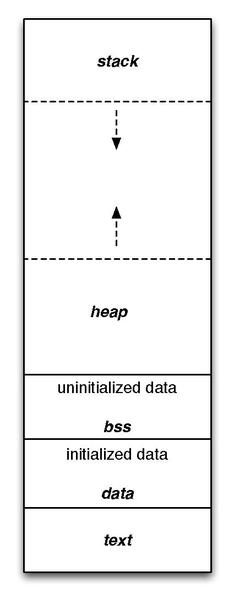
\includegraphics[scale=0.8]{stackHeap.jpg}
\centering
\end{figure}

Durante l'esecuzione un processo può trovarsi in diversi \textit{stati}. 
Gli stati possibili sono:
\begin{itemize}
	\item Nuovo (new): il processo è creato, ma non è ancora ammesso all'esecuzione.
	\item Pronto (ready): il processo può essere eseguito.
	\item In esecuzione (running): le sue instruzioni sono in esezuzione su un processore.
	\item In attesa (waiting): il porcesso non è esecuzione perchè sta aspettando un evento (es. input utente..).
	\item Terminato (terminated): il processo ha terminato l'esecuzione.
\end{itemize}

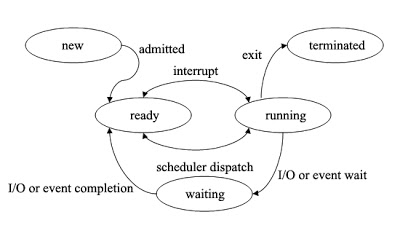
\includegraphics[scale=0.8]{processStateDiagram.jpg}

\subsubsection{Process Control Block}
Detto anche "Task Control Block", contiene le informazioni relative ad un processo:
\begin{itemize}
	\item Process state: ready, running...
	\item Program number (o PID): identifica il processo
	\item Program counter: contenuto del registro "istruzione successiva"
	\item Register: contenuto dei registri del processore
	\item Informazioni di scheduling: priorità, puntatori a code di scheduling..
	\item Informazioni relative alla gestione della memoria: memoria allocata al processo
	\item Informazioni di accounting: CPU utilizzta, tempo trascorso..
	\item Informazioni su I/O: dispositivi asseganti al processo, elenchi file aperti...
\end{itemize}
\begin{figure}[ht]
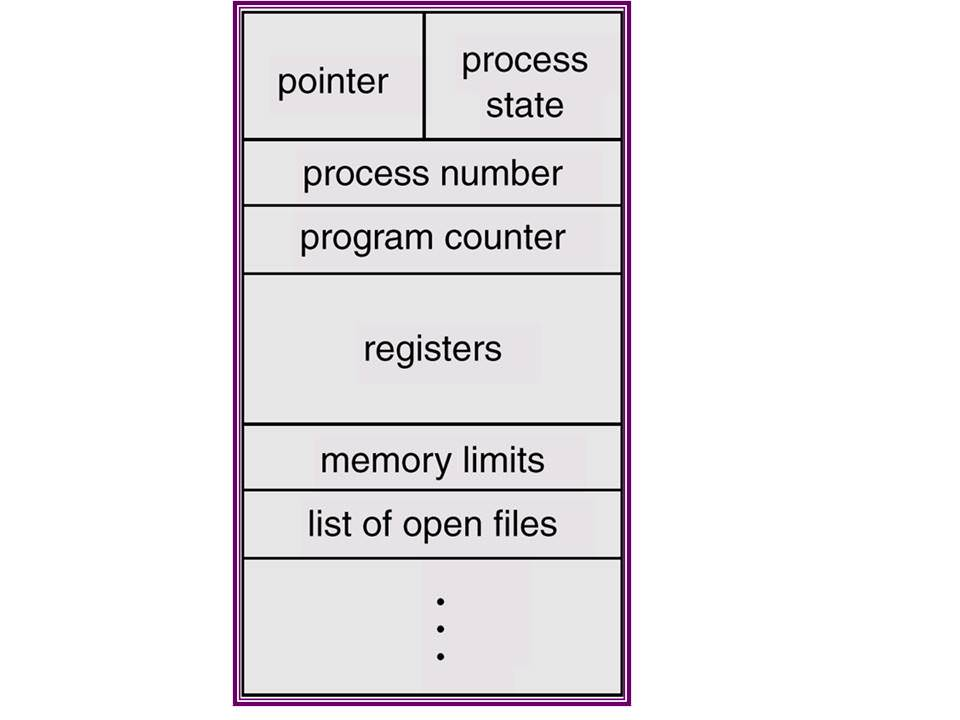
\includegraphics[scale=0.3]{ProcessControl.jpg}
\centering
\end{figure}

\subsubsection{Threads}
Fino ad ora abbiamo assunto che un processo abbia un singolo flusso di esecuzione sequenziale. Supponiamo che si possano avete molti program counter per un singolo processo:
\begin{enumerate}
\item 
\end{enumerate}

\subsubsection{Scheduling dei processi}
L'obiettivo dello scheduling dei processi è quello di massimizzare l'utilizzo della CPU. Una tecnica per fare questo è quella del \emph{Time-sharing}:

Lo scheduler dei processi sceglie il prossimo processo da eseguire tra quelli in stato ready.
Ci sono diverse code di processi:
\begin{itemize}
 \item Ready queue: processi residenti in memoria
\item Wait queue: diverse code per i processi in attesa
\end{itemize}
Durante la loro vita i processi migrano tra una coda e l'altra.
\\ \\
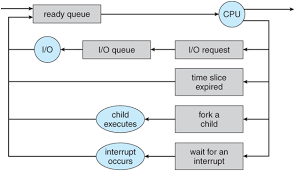
\includegraphics[scale=1.1]{processQueue.png}
\\ \\

Quando un SO decide che si deve cambiare processo, si ha la \textbf{commutazione di contesto} (o \textit{context switch}). Quando la CPU passa ad eseguire un processo diverso, il sistema operativo deve salvare lo stato del processo precedente, e caricare lo stato salvato del processo da rieseguire attaverso un context-switch.
Il PCB rappresenta il contesto di un processo. Il tempo necessario per il context switching è puro overhead: non viene eseguito alcun lavoro utile. Più è complesso l'SO, più è complesso cambiare processo per il context-switch.
\\ \\
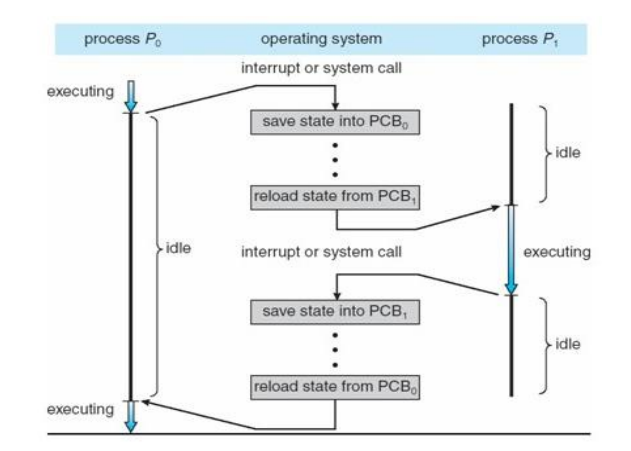
\includegraphics[scale=0.7]{context-switching.png}
\\ \\ 
\paragraph{Multitasking nei sistemi mobili} Alcuni sistemi mobili (es. le prime versioni di iOS) permettevano solo ad un processo di essere in esecuzione. Da iOS4 è possibile avere un processo in esecuzione in \textbf{foreground} (ha lo schermo a disposizione) e un certo numero di processi in esecuzione in \textbf{background} (senza schermo), ma con dei limiti.
Android ha molti meno limiti: i processi in background che vogliono effettuare delle elaborazioni devono creare opportuni \textit{servizi}, che:
\begin{itemize}
\item non hanno interfaccia utente
\item possono usare un ridotto contenuto di memoria
\item possono continuare a funxionare anche quando l'app in backgorund è sospesa
\end{itemize}
L'aumento di potenza dei sistemi mobili rende i loro OS sempre più simili a quelli non mobili.

\subsection{Operazioni sui processi}
\subsubsection{Creazione di processi}
Di solito nei sistemi operativi i processi sono organizzati in maniera gerarchica:
\begin{itemize}
\item un processo (padre) può creare diversi processi (figli) fino a creare un \textit{albero di processi}.
\item PORCODDIO PERCHECAZZO VA COSI VELOCE
\end{itemize}
Sistemi operativi diversi creano processi in modo diverso. Possono esistere diverse politiche di condivisione (padre e figlio condividono le risorse, solo alcune, nessuna), diverse politiche di creazione di spazio di indirizzi (il figlio è un duplicato del padre (stessa memoria e programma, oppure il figlio deve eseguire qualcos'altro) e ancora politiche di coordinazione padre/figli (il padre è sospeso finchè i figli non terminano, oppure eseguono in maniera concorrente).

Esempio: sistema UNIX
\begin{figure}[H]
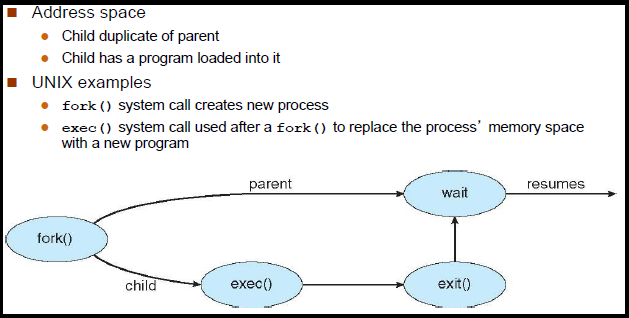
\includegraphics[scale=0.8]{UNIX-process.png}
\end{figure}

\section{lezione mancante}

\section{Scheduling della CPU}
Simulazioni e modellazione lo devo fare io da E-Learning.
\subsection{Algoritmi di scheduling della CPU}
Come anche per il resto dell'informatica, non esiste un solo algoritmo per svolgere questo compito. Ogni algoritmo ha diverse strategie di azione, e una CPU utilizza in modo intelligente questi algoritmi combinandoli anche tra di loro.

\paragraph{Concetti fondamentali}: lobiettivo della multiprograazione è massimizzare l'utilizzo della cpu. GLI ALGORITMI di scheduling sfruttano il fatto che di norma l'esecuzione di un processo è una sequenza di:
\begin{itemize}
	\item \textbf{Brust della CPU}:sequenza di operzaione di CPU.
	\item \textbf{Brust dell'I/O}: attesa del completamento di operazione I/O.
\end{itemize}
Un'efficente distribuzione dei brust è essenziale per la CPU.
\begin{figure}[H]
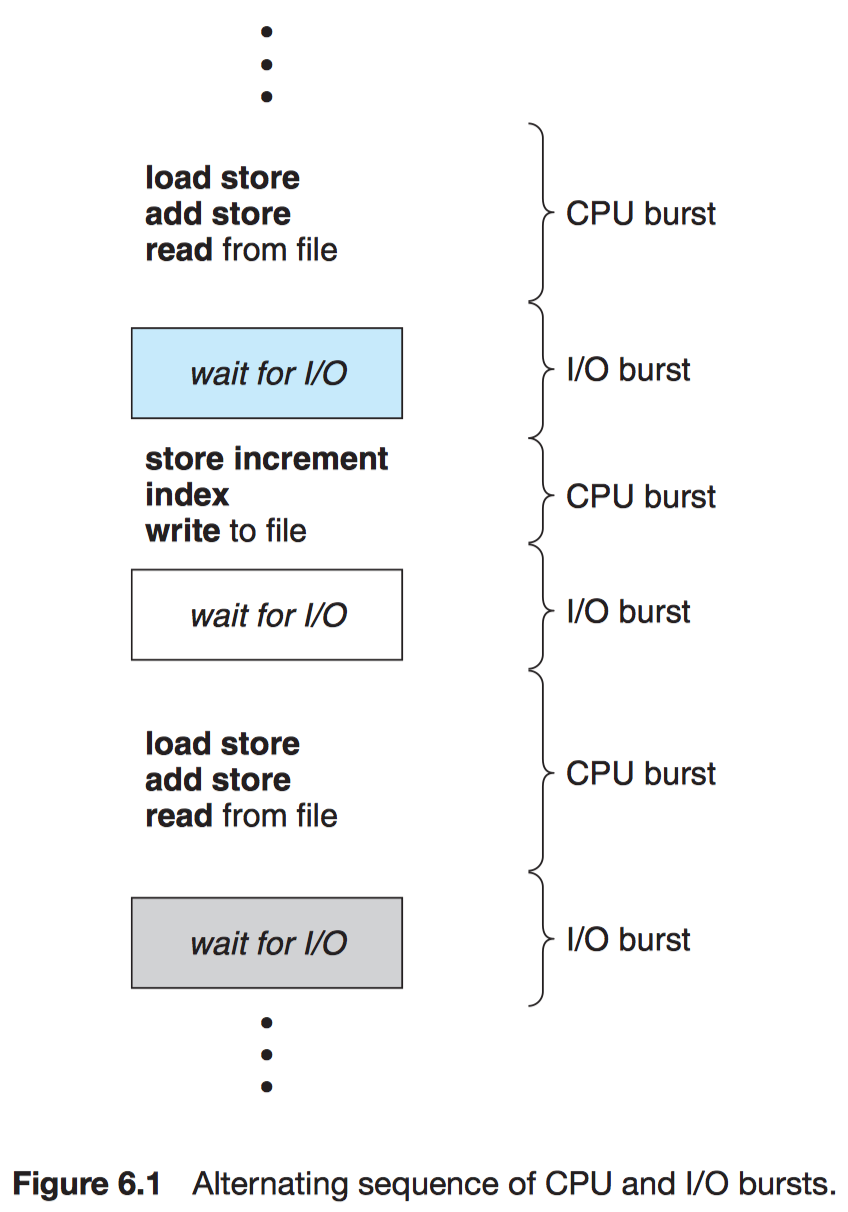
\includegraphics[scale=0.4]{burst.png}
\centering
\end{figure}

\paragraph{Distribuzione delle durate dei burst della CPU}
guardo slide per foto

\paragraph{Scheduler della CPU} Lo scheduler della CPU, o \textit{scheduler a breve termine}, seleziona un processo tra quelli nella ready queue (non per forza FIFO) ed alloca un core ad esso.
I riassegnamenti della CPU possono essere effettuati  in diversi momenti:
\begin{enumerate}
	\item quando un processo passa da running a waiting.
	\item qunado un processo passa da running a ready.
	\item quando un processo passa da waiting a ready.
	\item quando un processo termina.
\end{enumerate}
Non è detto che un sistema operativo faccia scheduling su tutte e quattro le situazioni.
Se il riassegnamento viene fatto solo nelle situazioni 1 e 4, lo schema di scheduling è detto \textit{senza prelazione} (\textbf{nonpreemptive} o cooperativo, altrimenti è detto \textit{con prelazione} (\textbf{preemptive}.
I processi cooperativi devono appunto collaborare: se volesse, un processo potrebbe tenersi il core occupato per tutto il tempo che desidera.
Lo schema di scheduling preemptive è più complicato da implementare ma è anche più sicuro:
\begin{itemize}
	\item che succede se due processi condividono dei dati?
	\item che succede se un processo sta eseguendo del codice in modalità kernel?
	\item che succede se un processo sta eseguendo un gestore degli interrupt?
\end{itemize}
\paragraph{Dispatcher} Il dispatcher passa effettivamente (fisicamente) il controllo della CPU al processo scelto dallo scheduler a breve termine:
\begin{itemize}
	\item Effettua il csmbio di contesto.
	\item Passa in modalità utente.
	\item Salta nel punto corretto del programma del processo selezionato (ossia dove era stato interrotto il processo).
\end{itemize}
La \textbf{latenza di dispatch} è il tempo impegato dal dispatcher per fermare un processo ed avviarne un altro.
\begin{figure}[H]
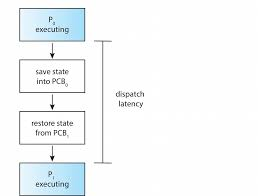
\includegraphics[scale=0.6]{dispatchLatency.jpg}
\centering
\end{figure}

\subsection{Criteri di scheduling}
Misure che servono per confrontare le caratteristiche dei diversi algoritmi (notare che non dioendono solo dall'algoritmo, ma anche dak tipo di carico).
I rincipali criteri sono:
\begin{itemize}
	\item \textbf{Utilizzo della CPU}: \% di tempo in cui la CPU è attiva (dovrebbe essere tra 40\% e il 90\% ).
	\item \textbf{Throughout}: \# di processi che completano l'esecuzione nell'unità di tempo (dipende dalla durata dei processi).
	\item \textbf{Tempo di completamento}: tempo necessario per completare l'esecuzione di un certo processo (dipende da molti fattori: durata del processo, carico totale...).
	\item \textbf{Tempo di attesa}: tempo trascorso dal processo nella ready queue (meglio del tempo di compèletamento , meno dipendente dalla durata del processo e dell'I/O).
	\item \textbf{tempo di risposta}: negli ambienti time-sharing, tempo trascorso tra l'arrivo di una richiesta al processo e la produzione della prima risposta, senza l'emissoine di questa nell'output.
\end{itemize}

\subsection{Algoritmi}
\subsubsection{Scheduling in ordine di processo} Chiamato anche \textbf{first-come-first-served} (o FCFS): la CPU viene assegnata al primo processo che la richiede.
\paragraph{Vantaggio}: è molto semplice da implementare (coda FIFO).
\paragraph{Svantaggio}: tempo di attesa medio può essere lungo (effetto "convoglio").
\begin{figure}[H]
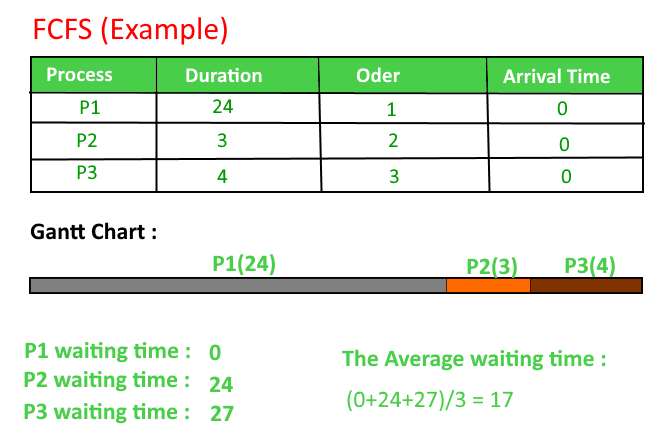
\includegraphics[scale=0.7]{FCFS.png}
\centering
\end{figure}
Ma nella figura, scambiando l'ordine dei processi la situazione può cambiare molto. Quindi dipende molto dall'ordine in cui arrivano i processi.

\subsubsection{Scheduling per brevità} Chiamato anche \textbf{shortest-job-first} (o SFJ): la CPU viene assegnata in base a l processo che ha il successivo CPU burst più breve.
\paragraph{Vantaggio}: minimizza il tempo di attesa medio (è \textbf{ottimale}).
\paragraph{Svantaggio}: non esiste modo per sapere qual è il processo che avrà il CPU burst più breve! Visto che questo non è possibile nella pratica, si può solo "stimare".
\\ \\ 
inserisco il paragone tra FCFS  e SFJ
\\ \\
Come stimo il burst di un processo?
\paragraph{Idea:} registrare la lunghezza dei CPU burst precedenti ed applicare una \textbf{media esponenziale}:
\begin{enumerate}
	\item $t_n$ = durata effettiva dell'n-esimo burst.
	\item Sia $\alpha$ un valore compreso tra 0 e 1.
	\item Sia $T_{k+1} = \alpha t_k + (1 - \alpha ) T_k$
	\item La media esponenziale è data da $T_{n+1 }$
\end{enumerate}
La versione preemptive è chiamata \textbf{shortest-remaining-time-first}.
Il parametro $\alpha$ "bilancia" il peso della storia recente vs. storia passata (di solito si usa $T = 0.5$).
Se $\alpha = 0$, la storia non conta, torna il FCFS
Se $\alpha = 1$, conta solo la durata dell'ultimo burst.
\\ \\
Con il shortest-remainig-time-first abbiamo che il tempo di attesa medio di un processo è:
\begin{equation}
istante \medspace terminazione  \medspace processo - (tempo \medspace di \medspace arrivo  + durata \medspace burst)
\end{equation}
\\ \\
ci ficco la foto delle slide
\\ \\

\subsubsection{Scheduling circolare}
In uno scheduling circolare, o \textbf{round-robin} (RR) abbiamo che:
\begin{itemize}
	\item Ogni processo ottiene una piccola quantità fissata di tempo di CPU
	\item trascorso tale tempo il processo viene interrotto e messo in fondo alla ready queue
	\item la ready queue è trattata come un buffer circolare
\end{itemize}
Se ci sono $n$ processi nella ready queue e il quanto temporale è $q$, allora ogni processo ottiene 1/n di tempo di CPU e nessun processo attende più di q*(n-1) unità di tempo nella ready queue.
Per effettuare la prelazione del processo corrente si effettua un interrupt del timer ogni q di tempo.
\\ \\
foto dello scheduling circolare
\\ \\


\textbf{Confronto tra algoritmi di scheduling}
\begin{figure}[H]
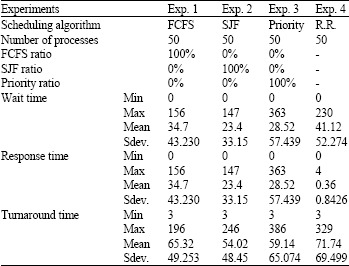
\includegraphics[scale=8]{scheduling-vs.jpg}
\centering
\end{figure}

\end{document}
